\chapter{\texorpdfstring{\MakeUppercase{Technology Setup}}{Technology Setup}}

A major driving principle of the presented work is that the methodology
needs to be scalable. One reason for difficulties in implementing fault
detection and diagnostic algorithms and other optimization methods is
that there is a significant amount of initial investment necessary. This
initial investment can also be cost prohibitive. 

In more complex schemes, it may be necessary to install additional
sensors that are typically not available in commercial HVAC systems.
Along with the sensor cost, there is the cost to tie the sensors into the
BAS. The updated logic will likely be coded by a controls contractor,
adding more cost. On a large campus, this reprogramming can also take a
significant amount of time to complete. 

Another issue is that of risk. There is the risk that if the controls do
not function properly and are too complex for the current building
operator, the controls cannot be easily removed and set back to the 
previous state. 

\section{Proposed Setup}

In the proposed setup, the amount of change to the existing BAS is
minimal. The control logic remains exactly the same. A small executable
script can be installed on the BAS computer that can host code that will
send an HTTP request to a remote server holding the historical data and
the optimization methods. 


\figref{} \ref{fig:NetworkFlow} shows potential information flow. Over
any period, historical trend data representing the system is stored
in a server. This data may come in one large sync or potentially occur
daily or sub-daily. Once enough data has been stored on the server, a
client BAS computer (potentially one of many) can make an HTTP request
that will essentially carry information related to the current time and
what equipment the request is for. Each AHU will have a unique
identifier that the main web server understands. 

The web server will implement the methods described in this document and
will send a response back to the client with the setpoints for the
system that will be near-optimal in a steady-state sense, given the
expected conditions at the building and individual zones. 

\subsection{Standards for Transmission}

Standards for the format of information transfer are critical for rapid
adoption. An Application  Program Interface (API) is the public
interface of methods and routines that allow third-party programmers to
develop programs from the base building blocks. 

Another important point of consideration is the format of the data
actually being transferred. In the software industry, there are several
types of data exchange formats, two popular ones being JavaScript Object
Notation (JSON) and Extensible Markup Language (XML). 

The advantage of JSON over XML is that JSON requires fewer characters to
describe simple objects. Unlike XML, it does not support explicit schema
definition. 

\begin{figure}
\begin{tikzpicture}

\node [anchor=center,draw] (BASComputer) at (0,0) {\includegraphics[width=3cm, height=3cm]{Images/Desktop_computer_clipart_-_Yellow_theme-MPEdits.png}};

\node [anchor=center,draw] (Server) at (7cm, 0) {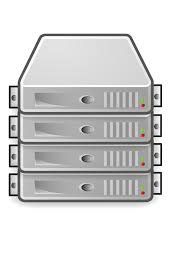
\includegraphics[width=3cm, height=3cm]{Images/serverImage.jpg}};

\draw [->, out=25, in=155, thick,anchor=center ] (BASComputer) to node
    [yshift=1cm, align=center] {HTTP request \\ \(\approx\)5-15 min} (Server);

\node [above=of Server] {Web Server};

\node [right=of Server, align=left] {Historical data at \\ any syncing interval};

\draw [->, out=225, in=315, thick, ] (Server) to node [yshift=1cm, align=center] {Optimal Setpoints} (BASComputer);



\end{tikzpicture}    
\caption{Diagram of networking flow.}
\label{fig:NetworkFlow}
\end{figure}


\subsection{Advantages to Proposed System}

There are several key advantages to a system similar to the proposed:

\begin{enumerate}
    \item No real-time data transmission. Managing the networking of
        large BAS systems is difficult enough as is. It is not feasible
        for a single server to handle live streams of BAS point
        information from thousands of buildings. 

    \item The system can be added or removed quickly and without
        side-effects. Because the logic lives at an abstraction level
        above the BAS code, no changes to the system need to be made
        locally. 

    \item Routines only have to be added once for different equipment
        and setup types, allowing the same methods to expand to many
        different buildings. 
\end{enumerate}

The equipment can be separated by project, and a call such as

\url{https://domain/GetEquipmentForProject/?ProjectId={Project-Id}}

The interface for receiving the optimal setpoints could have a url
similar to 

\url{https://domain/setpoints/?id={Equipment-Id}\&{time=Datetime}}

\section{Prototype Information}

The proposed system was implemented in the software tool
\textit{Implementer}, a web application developed at the Energy Systems
Laboratory. Implementer can analyze trend data from any system that has
an ability to store timestamp value pairs and allow access to them. 

The current systems supported by Implementer include:

\begin{itemize}
    \item Alerton
    \item Andover Continuum
    \item Automated Logic
    \item Delta Controls Historian
    \item Emerson Ovation
    \item Honeywell Hoboware
    \item Johnson Controls Metasys
    \item Reliable Controls
    \item Siemens APOGEE
    \item TAC I/NET Seven
    \item TAC I/A Series
    \item Trane Tracer
    \item Tridium Niagara 
\end{itemize}

Before this process can begin, the sensors will need to be mapped in a
way that the server can understand. 

In Implementer, trends are given meaning through the use of
\textit{Labels}. Labels are similar to the concept of tagging that is used
in other systems, such as a system that implement Project Haystack. 

Trends can receive labels in several ways. For trends in air handling
units, the label can automatically be derived from the type of sensor and
location on a schematic. A sample schematic from the NCTM project is
shown in \figref{} \ref{fig:AHUSchematic}. For example, a temperature
sensor that is at the outlet of the air handling unit, unaffected by any
other temperature affecting device, is defined to have the supply air
temperature label. 

Labels can also be created manually. \figref{} \ref{fig:CustomLabels}
shows how all \textit{AUX TEMP} trends from the different fan powered
VAV (FPVAV) units are labeled as \textit{DischargeTemps}.

An entire site or building is organized into Containers and a
hierarchy of components. A building container is a parent to air
handling unit containers, and air handling unit containers are parents
to terminal unit containers. \figref{} \ref{fig:ContainerHierarchy}
shows a portion of the hierarchy for the NCTM project.

\begin{figure}
\centering
\includegraphics[scale=0.5]{Images/SampleAHUSchematic.PNG}
\caption{Sample AHU schematic for AHU-2-2 in the NCTM building.}
\label{fig:AHUSchematic}
\end{figure}

\begin{figure}
\centering
\includegraphics[scale=0.75]{Images/CustomLabels.PNG}
\caption{Custom labels setup, showing how all \textit{AUX TEMP} trends
are associated to the label \textit{DischargeTemps}. }
\label{fig:CustomLabels}
\end{figure}

\begin{figure}
\centering
\includegraphics{Images/ContainerHierarchy.PNG}
\caption{Container Hierarchy for NCTM.}
\label{fig:ContainerHierarchy}
\end{figure}

In order to complete the optimization, the inputs and functions for the
various trends need to be input. It is proposed that the use of a
container hierarchy, labels or tags, and custom equations be used to
develop the system.

Implementer uses something called container properties, and one of the
properties can be set to a JSON object that contains all the necessary
pointers to values or custom equations.

The necessary inputs for the AHU container would be 
\begin{enumerate}
    \item Exponent for the fan curve, \(n\)
    \item Prediction function for \(\mat{}\) 
    \item Design fan power \(\dot{W}_{design}\)
    \item Design AHU flow 
\end{enumerate}
For the children terminal unit containers, if a series fan powered
terminal unit is assumed, the necessary inputs will be
\begin{enumerate}
    \item Zone temperature setpoint prediction
    \item Zone load prediction
    \item Plenum temperature prediction
    \item Minimum damper position
\end{enumerate}

Parameters needed for the optimization are input for each container in
the container details portion of Implementer. The settings are formatted
in JSON, as shown in \figref{} \ref{fig:JSONOptions}. The properties
include options such as pointers to how the mixed air temperature
should be calculated, the maximum supply humidity ratio, and the
assumed part load ratio fan exponent. 

These pointers can be a static value, another property, an actual
trend from the building automation system, or a custom equation built up
using the powerful functions available in Implementer.

\begin{figure}
\centering
\begin{lstlisting}[language=json]
OptSATGenPoint = 
{"MATPrediction":"MAT Prediction",
"VDesign":"VDesign",
"FanExponent":2,
"WDesign":"WDesign",
"MaxHumidityRatio":0.009,
"Name":"Optimal SAT-Ex-2",
"BoundTermUnitProp":"SeriesBoxOptions",
"SATEnergySelector":"SAT"};
\end{lstlisting}
\caption{JSON options for the second floor air handling units. }
\label{fig:JSONOptions}
\end{figure}

Any calculation  from the optimization analysis can be output as a trend
in Implementer and can be plotted and visualized using any of the tools
available. 






